\documentclass{article} % For LaTeX2e
\usepackage{nips15submit_e,times}
\usepackage{hyperref}
\usepackage{url}
\usepackage{graphicx}
%\documentstyle[nips14submit_09,times,art10]{article} % For LaTeX 2.09


\title{Assignment 2 for Applied Machine Learning 15 Fall}


\author{
Jingyuan Liu\\
AndrewId: jingyual\\
\texttt{jingyual@andrew.cmu.edu} \\
}


\newcommand{\fix}{\marginpar{FIX}}
\newcommand{\new}{\marginpar{NEW}}


\nipsfinalcopy % Uncomment for camera-ready version


\begin{document}
\maketitle


\section{Part A}


\subsection{Question 1: Show three decision trees on different datasets}
In this question, I trained decision trees seperately on three different
datasets. Specifically:\\
(1) The Figure \ref{fig:titanic} shows the decision tree trained with
``titanic.arff'' datasets.
\begin{figure}[h]
\begin{center}
\fbox{\rule[-.5cm]{0cm}{4cm}
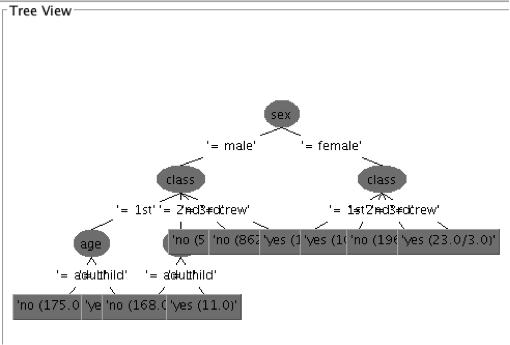
\includegraphics{pic/titanic.png}
}
\end{center}
\caption{titanic.arff dat trained tree.}
\label{fig:titanic}
\end{figure}

(2) The Figure \ref{fig:titanic-age-numeric} shows the decision tree
trained with ``titanic-age-numeric.arff'' datasets.
\begin{figure}[h]
\begin{center}
\fbox{\rule[-.5cm]{0cm}{4cm}
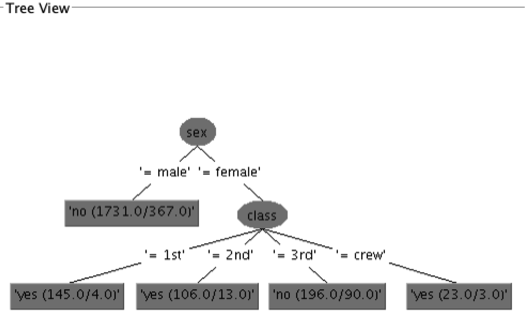
\includegraphics{pic/titanic-age-numeric.png}
}
\end{center}
\caption{titanic-age-numeric.arff dat trained tree.}
\label{fig:titanic-age-numeric}
\end{figure}

(3) The Figure \ref{fig:titanic_noise} shows the decision tree
trained with ``titanic\_noise.arff'' datasets.
\begin{figure}[h]
\begin{center}
\fbox{\rule[-.5cm]{0cm}{4cm}
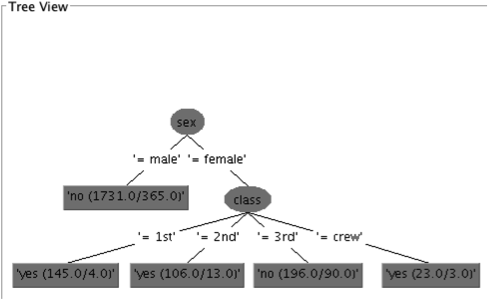
\includegraphics{pic/titanic_noise.png}
}
\end{center}
\caption{titanic\_noise.arff dat trained tree.}
\label{fig:titanic_noise}
\end{figure}


\subsection{Question 2: Compare results of Figure \ref{fig:titanic} and
Figure \ref{fig:titanic-age-numeric}}
The results and the learned decision trees ars quiet different on these two
different datasets. According to the figure drew from weka, we can see that in
Figure \ref{fig:titanic}, there are more classification rules than in Figure
\ref{fig:titanic-age-numeric} for the ``male'' subclass. Besides, the Figure
\ref{fig:titanic} shows that there existed a classification hierachy more than
Figure \ref{fig:titanic-age-numeric}, the ``age''.\\
I think it is almost impossible for the two different datasets to generate the
same learning tree, because compared with numeric data, the nominal data lose
some ``information'', like ``order'' and ``distance''. What is more, the nominal data
would somehow create more classification rules than numeric data.\\
The J48 settles different different models because those two datasets contains
different amout of ``information''.


\subsection{Question 3: Compare results of Figure \ref{fig:titanic-age-numeric} and
Figure \ref{fig:titanic_noise}}
As the the two figures showed, the learning results are different. For Figure
\ref{fig:titanic-age-numeric}, the ``male'' classfication value is ``no (
1731/367)'', while for Figure \ref{fig:titanic_noise}, the corresponding value
is ``no (1731/365)''. The noise would slightly influence the classification
performance for some instance in the ``male'' subclass.\\
I think, the noise-trained tree would make mistakes on instances with value ``no
(1731/366)''. Those instances with the related values falling into the
difference gap of the two learned tree would lead the classification tree make
mistakes.


\section{Part B}
Just see the SetupSearchData.py and output.csv.


\end{document}
